\documentclass[runningheads]{llncs}

\usepackage{graphicx}
\usepackage{amsmath,amssymb}
\usepackage{booktabs}
\usepackage{url}
\usepackage{hyperref}
\usepackage{tabularx}

\begin{document}

\title{Evaluating Rule Compliance and Decision Traceability in a Social Assistance Eligibility Prototype}
\titlerunning{Rule Compliance and Decision Traceability in Sociovault}

\author{Dzaky Ahsanal Khuluq \and Annisa Nailatul Izzah}
\authorrunning{D. A. Khuluq and A. N. Izzah}

\institute{Electronic Engineering Polytechnic Institute of Surabaya, Surabaya, Indonesia\\
\email{humas@pens.ac.id}\\
\url{https://it.pens.ac.id/}}

\maketitle

\begin{abstract}
The distribution of social assistance relies on consistent and traceable citizen eligibility assessments, whereas manual or decentralized examinations risk producing ununiform and uncorrectable evaluations. This study evaluates the Sociovault prototype, a Flask-based web application running a three-stage rule engine for a single assistance program: data completeness checks, four-criterion evaluations, and final officer confirmation. This research aims to test whether the system's recommendations and rationales follow defined rules, and whether decisions can be traced and corrected. The method used is rule compliance testing against a rule matrix with 60 synthetic cases (Test 1) along with boundary value analysis and duplicate verification (Test 2). The results show label compliance of 100\% and rationale compliance of 100\% across all evaluated scenarios.

\keywords{Sociovault \and social assistance \and eligibility verification \and rule engine \and decision traceability \and rule compliance}
\end{abstract}

\section{Introduction}

Social assistance programs are one form of government support intended to help people in need~\cite{uu11_2009,perpres95_2018}. In their implementation, examining applicant data is an important step in ensuring that eligibility recommendations are based on available information and predefined criteria. This examination process needs to be conducted systematically so that each recommendation can be explained using the available data. Therefore, a social assistance eligibility assessment prototype can be used to help evaluate the consistency of applicant data with established rules and provide explanations for the recommendations generated by the system.

Several risks need to be considered during the eligibility assessment process, including incomplete data, duplicate applications, and decisions that are not accompanied by verifiable explanations~\cite{uu27_2022}. Incomplete data may cause the system to produce recommendations whose validity cannot yet be determined, while duplicate data may lead to inconsistencies during the assessment process. Furthermore, recommendations without adequate explanations may make it difficult for officers to understand the basis of a decision and identify information that needs to be corrected. Therefore, the system needs to provide verification and explanation mechanisms that allow each recommendation to be traced to the data and rules used.

One approach that can be applied is rule-based eligibility, which assesses eligibility using a predefined set of rules and criteria. This approach needs to be supported by decision traceability, which refers to the ability to trace the relationship between input data, applied criteria, and the recommendations generated. Traceability also includes recording criteria versions and data changes that may affect assessment results. Through these mechanisms, errors can be examined, inconsistent data can be corrected, and recommendations can be recalculated based on the changes made. When the available information is insufficient, the system should flag the case for further verification rather than immediately concluding that an applicant is ineligible without a clear rule-based justification.

Based on these issues, this study focuses on evaluating rule compliance and decision traceability in a social assistance eligibility assessment prototype. The evaluation examines whether the recommendations and explanations generated by the system are consistent with the applied criteria, including tests involving incomplete data, duplicate applications, threshold values, and data corrections. This study is expected to determine whether the prototype applies its rules consistently and provides decision explanations that can be traced and reviewed. However, the evaluation results demonstrate only the system's compliance with the tested prototype specifications and do not directly establish the fairness or validity of social assistance policies. The final decision regarding assistance eligibility remains the responsibility of the authorized parties.

\section{Related Work}

This literature search is limited, as it was conducted with only a few queries. The gap statements in Subsection~\ref{subsec:gap} need to be confirmed with a systematic search in academic databases such as Scopus, IEEE Xplore, or the ACM Digital Library.

\subsection{Rule-Based Eligibility and Transforming Policies into Decision Models}

Research on social service eligibility automation emphasizes that eligibility rules are often embedded in policy documents, making them difficult to translate into executable logic. Wei et al. proposed a semi-automated approach using AI, NLP, and knowledge graphs to transform eligibility policy documents into executable and interpretable decision models, using standard DMNs and the FEEL language~\cite{wei2022envisioning}. [This paper was published in December 2022 by researchers such as Vanessa Lopez.] This approach is relevant to Sociovault because it separates the rules from the application code, while the Sociovault engine still embeds criteria in Python functions.

Industry sources also discuss a similar approach, separating eligibility logic into auditable decision models~\cite{progress_software}. However, these sources are software marketing materials and are not treated as scientific evidence in this paper.

Sociovault's distinction from these approaches lies in its scope. Sociovault does not separate criteria into a declarative format. The criteria are stored in the \texttt{help\_program} table and evaluated by the \texttt{run\_verify} function, so their compliance needs to be tested directly.

\subsection{Explainable and Auditable Decision Support for Public Services}

The literature on automated public assistance systems increasingly emphasizes auditability, not just interpretability. Sunny shows that explanations generated by eligibility systems often do not reflect the actual legal basis and proposes a framework that links explanations to requirements ontology and solver checks~\cite{sunny2025neuro}. Similar research from the same group suggests that explanations to applicants should contain the legal basis for decisions to be verifiable by stakeholders~\cite{sunny2024legal}. [ALLEN DANIEL SUNNY, IDO SIVAN-SEVILLA, 6 may 2026.]

Both of these studies work at the legal basis level, using the CalFresh program in the United States as the object of study. Sociovault works at a different level: its output is a detailed check per criterion (value, threshold, and eligibility status), not a legal argument. Thus, the relevant question for Sociovault is whether the details are consistent with the rules used, not whether the rules are legally valid.

\subsection{Deduplication and Recipient Identity Matching}

The issue of duplicate recipients has long been recognized in the administration of aid. A 1978 GAO report compared recipient data across jurisdictions using Social Security Numbers (SSNs) as the sole identifier; it found that some matches occurred due to incorrect or missing SSNs, as well as a lack of uniform data storage formats~\cite{gao1978duplicate}. These findings underscore the importance of identity quality in the deduplication process.

Rule-based approaches have also long been employed by government agencies. A 1987 circular from the California Department of Health described matching names and dates of birth to detect dual program participation, with a rule requiring an exact match for names~\cite{california1987match}. A subsequent 1994 circular outlined procedures for verifying potential duplicates using verified identification numbers~\cite{california1994letter}. Both examples demonstrate that matching based on names and dates of birth yields candidates requiring human review, rather than serving as a final determination.

More modern approaches utilize ``entity resolution'' that is tolerant of typos. The OpenG2P Deduplication Service combines attributes---such as name, address, and date of birth---to identify potential duplicates, with support for additional methods like fingerprinting or facial recognition~\cite{openg2p_dedup}. A requirements specification for the openIMIS project proposes a deduplication module featuring fuzzy matching and audit logs for all deduplication activities~\cite{openimis2022algorithm}. Deduplication guidelines from the Philippines also establish multi-tiered deduplication procedures across different offices [No.~18, Series of 2020]~\cite{dswd2020guidelines}. Harmonizing data systems across organizations has also proven essential in broader humanitarian and emergency cash transfer programs~\cite{owino2020harmonising}.

Sociovault only prevents duplication based on an exact match of the national identification number (NIK); similarity-based matching has not yet been implemented. Consequently, Sociovault functions more like a unique-key approach than a true entity resolution system. For this reason, the issue of duplication is not addressed in this paper. This limitation should be explicitly stated in the section on study limitations.

\subsection{Identity Data Quality and Handling of Missing Data}

In the literature on deduplication for assistance programs, missing or incorrect data is often a primary source of error. A GAO report~\cite{gao1978duplicate} indicates that some beneficiary files either lack a Social Security Number (SSN) or contain an incorrect one. Based on the literature regarding the handling of missing data in eligibility decision systems, the common policy is to treat empty data fields as items requiring further review---rather than immediately categorizing them as ``ineligible''---to avoid the erroneous exclusion of legitimate beneficiaries. Sociovault classifies empty mandatory fields as ``requiring review'' rather than ``ineligible.'' While this approach aligns with the principles outlined in this research guide, it should be compared against other practices before it can be claimed to be superior.

\subsection{Sociovault's Position Relative to Previous Studies}
\label{subsec:gap}

Table~\ref{tab:comparison} compares Sociovault with the reviewed studies and sources across relevant dimensions.

\begin{table}[htbp]
\caption{Comparison of Sociovault with related sources}
\label{tab:comparison}
\centering
\begin{tabular}{p{2.2cm}p{2.6cm}p{2.6cm}p{2.6cm}p{2.0cm}}
\hline
\textbf{Source} & \textbf{Main Focus} & \textbf{Identity Matching} & \textbf{Decision Traceability} & \textbf{Measurable Testing} \\
\hline
Wei et al.~\cite{wei2022envisioning} & Policy-to-decision model & Not discussed & Discussed as an objective & Not visible in abstract \\
Sunny~\cite{sunny2025neuro} & Explanation vs law & Not discussed & Explanation vs legal basis & Case evaluation \\
GAO~\cite{gao1978duplicate} & Beneficiary deduplication & SSN only & Not discussed & Audit analysis \\
California~\cite{california1987match,california1994letter} & Name and DOB matching & Name and date of birth & Procedure letter & Not visible \\
OpenG2P~\cite{openg2p_dedup} & Entity resolution & Fuzzy matching & Not discussed & Not visible \\
Sociovault & Prototype eligibility verification & Unique NIK, dual verification constraints & Criteria-by-criteria check details, mandatory notes & Planned (Section~4) \\
\hline
\end{tabular}
\end{table}

The contribution that can be stated with limitation is the evaluation of rule engine compliance and reason traceability on a single prototype. The claim that this approach is superior to previous studies cannot yet be made, as there is no measurable comparison.

\section{Methodology}

\subsection{Program and Criteria Sources}

This research selects one assistance program from the three programs available in the initial data (\texttt{seed.py}). The selected program is Program A. The prototype was implemented using the Flask web framework~\cite{flask_doc} with SQLAlchemy ORM~\cite{sqlalchemy_doc}. The program criteria used are presented in Table~\ref{tab:criteria}.

The figures above represent prototype assumptions derived from initial data rather than official institutional criteria. This document must be replaced with applicable program regulations before being used for validity claims. Consequently, all the criteria thresholds above are established purely as independent simulation test scenarios to evaluate rule engine performance within the developed system prototype.

\begin{table}[htbp]
\caption{Criteria of the selected assistance program}
\label{tab:criteria}
\centering
\begin{tabular}{lll}
\hline
\textbf{Criteria} & \textbf{Threshold} & \textbf{Source} \\
\hline
Maximum Income & $\leqslant$ Rp 2,000,000 (Program A example) & Initial data \texttt{seed.py} \\
Minimum Dependents & $\geqslant$ 2 & Initial data \texttt{seed.py} \\
Maximum Assets & $\leqslant$ Rp 15,000,000 & Initial data \texttt{seed.py} \\
Maximum Welfare Decile & $\leqslant$ 3 & Initial data \texttt{seed.py} \\
\hline
\end{tabular}
\end{table}

\subsection{Status Diagram}

The verification status consists of two stages: automated status from the rule engine and final status from the officer. The following diagram represents this workflow based on the logic in \texttt{app/verifikasi/engine.py}:

\begin{figure}[htbp]
\centering
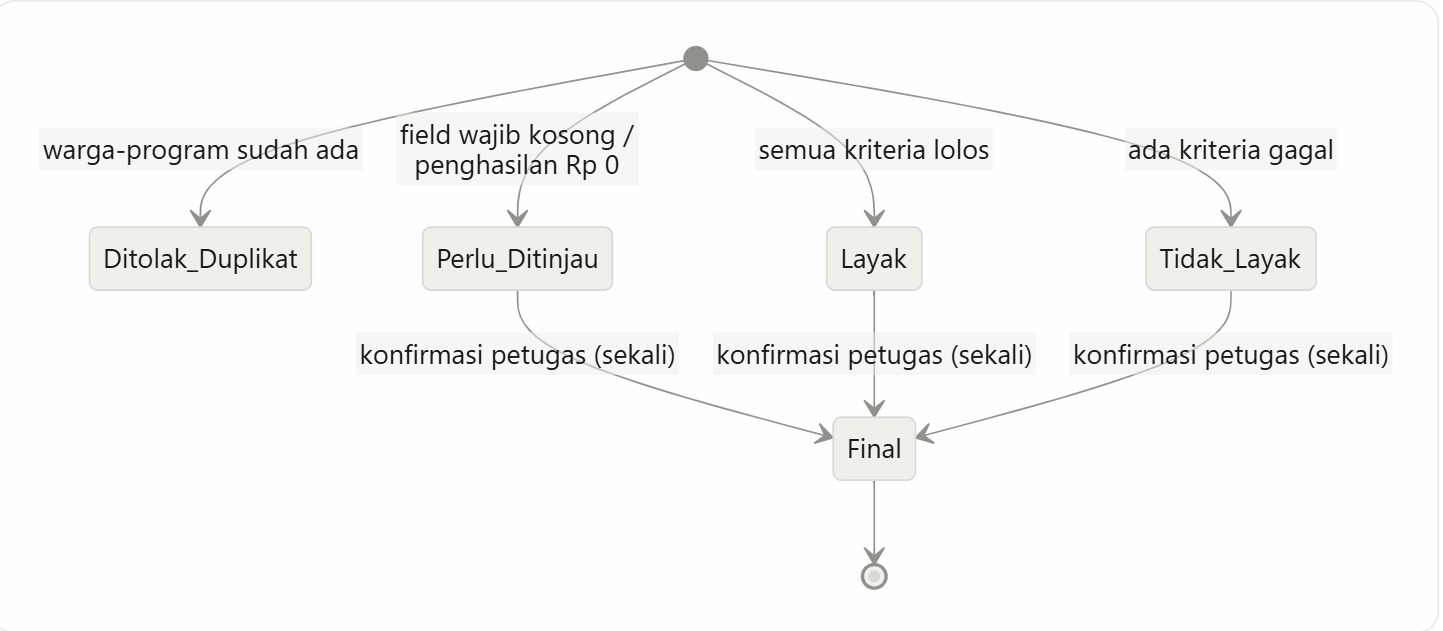
\includegraphics[width=0.92\textwidth]{status_diagram_fig.png}
\caption{Verification status workflow.}
\label{fig:status_diagram}
\end{figure}

\subsection{Initial Status, Action, Role, and Final Status Matrix}

Table~\ref{tab:workflow_matrix} presents the verification workflow rules matrix.

\begin{table}[htbp]
\caption{Verification workflow rules matrix}
\label{tab:workflow_matrix}
\centering
\begin{tabular}{p{2.7cm}p{2.2cm}p{2.5cm}p{2.6cm}p{2.0cm}}
\hline
\textbf{Initial Status} & \textbf{Action} & \textbf{Allowed Role} & \textbf{Final Status} & \textbf{Description} \\
\hline
No verification & Run verification & Administrator, verification officer & \texttt{layak}, \texttt{tidak\_layak}, or \texttt{perlu\_ditinjau} (automatic) & Calculated by engine \\
No verification & Run verification & Citizen & Rejected & Restricted by \texttt{role\_required} \\
Verified (\texttt{layak} or \texttt{perlu\_ditinjau}) & Re-run verification & Anyone & Rejected (\texttt{AlreadyVerifiedError}) & Duplication not allowed \\
Verified (\texttt{tidak\_layak}) & Re-run verification & Anyone & Rejected (\texttt{AlreadyVerifiedError}) & History already exists \\
Inactive program & Run verification & Anyone & Rejected (\texttt{ValueError}) & Program is inactive \\
Empty final status & Final confirmation & Administrator, verification officer & \texttt{layak}, \texttt{tidak\_layak}, or \texttt{perlu\_ditinjau} (final) & Mandatory notes \\
Filled final status & Re-confirmation & Administrator, verification officer & Rejected & Single confirmation only per route \\
\hline
\end{tabular}
\end{table}

Based on \texttt{engine.py}, there is no route to delete verification; re-verification for the same citizen and program pair is blocked to prevent data duplication.

\subsection{Verification Rules and Output Rationale}

The engine executes three sequential stages:
\begin{enumerate}
\item \textbf{Data completeness.} If a mandatory field is empty, the status is set to ``\texttt{needs\_review},'' and a list of the missing fields is recorded in the summary.
\item \textbf{Anomalies.} If income is Rp 0, the status is set to ``\texttt{needs\_review},'' with the rationale that a field survey is required.
\item \textbf{Criteria assessment.} Four criteria are evaluated: $\text{income} \le \text{threshold}$, $\text{dependents} \ge \text{threshold}$, $\text{assets} \le \text{threshold}$ (if defined), and $\text{decile} \le \text{threshold}$ (if defined). If all criteria are met, the status is ``\texttt{eligible}''; if any criterion fails, the status is ``\texttt{ineligible}.''
\end{enumerate}

Each result includes a ``\texttt{check\_details}'' object containing the value, threshold, pass/fail status, and a summary. These details serve as the basis for verifying the validity of the rationale during Test 1.

\subsection{Decile Estimation}

If a citizen does not yet have a decile value, the system calculates it using the following heuristic rule. Per capita income is calculated as income divided by $(\text{number of dependents} + 1)$. This value is mapped into ten classes, with an initial threshold of Rp 600,000 per capita for decile 1. The class can then be increased or capped by asset indicators, namely vehicle ownership, building area, electricity capacity, asset value, and housing status. This rule is not an official model and has not been validated. The decile value stored in the citizen's record always overrides the automated calculation result.

\subsection{Duplicate Data Prevention and Correction}

Prevention is implemented across three layers: a unique NIK key in the citizen table, a unique constraint on citizen and program pairs in the verification table, and a check for existing verification records within the engine. Name or date of birth similarity matching is not implemented. Citizen data correction is performed through data editing, whereas a new verification can only be executed for citizen--program pairs that do not yet have a verification history.

\subsection{Evidence of Requirements}

In the absence of field evidence from observations, interviews, or procedural documents, the problems addressed in this study are stated as prototype requirements and test scenarios rather than institutional findings.

\section{Experimental Design}

\subsection{Test 1: Rule Compliance (Mandatory)}

\textbf{Dataset:} 60 synthetic cases with unique synthetic identities (distinct synthetic NIKs for each case to prevent duplicate verification rejection), divided into three reference categories established prior to system execution as shown in Table~\ref{tab:test1_composition}.

\begin{table}[htbp]
\caption{Composition of the 60 synthetic test cases for Test 1}
\label{tab:test1_composition}
\centering
\begin{tabular}{p{3.2cm}cp{7.2cm}}
\hline
\textbf{Reference Category} & \textbf{Count} & \textbf{Case Description / Examples} \\
\hline
Eligible (\texttt{layak}) & 20 & Meets all Program A criteria (e.g., income Rp 1,500,000, dependents 3, assets Rp 5,000,000, decile 2). \\
Ineligible (\texttt{tidak\_layak}) & 20 & 15 single-criterion failure cases (4--5 cases per failed criterion: income, dependents, assets, or decile) and 5 multi-criteria failure cases ($\ge 2$ failed criteria). \\
Needs Review (\texttt{perlu\_ditinjau}) & 20 & Undecidable cases requiring officer review: 10 cases with empty mandatory fields (NULL) and 10 anomaly cases with Rp 0 income. \\
\hline
\end{tabular}
\end{table}

\noindent\textbf{Procedure:}
\begin{enumerate}
\item Establish the reference label and expected rationale for each of the 60 synthetic cases prior to system execution.
\item Execute all 60 cases through the prototype verification engine (\texttt{app/verifikasi/engine.py}) using isolated citizen--program pairs and record the resulting \texttt{status\_otomatis}, summary rationale, and \texttt{detail\_pengecekan}.
\item Compare the system-generated status and rationale against the reference label and expected failure/review conditions. A rationale is considered compliant if the failed criteria or the conditions triggering \texttt{perlu\_ditinjau} accurately reflect the input case data.
\end{enumerate}

\noindent\textbf{Metrics and Evaluation Results:} The evaluation measures label compliance, rationale compliance, false acceptances (reference \texttt{tidak\_layak} classified as \texttt{layak}), false rejections (reference \texttt{layak} classified as \texttt{tidak\_layak}), and premature automated decisions on review cases (reference \texttt{perlu\_ditinjau} classified as \texttt{layak} or \texttt{tidak\_layak}). The results of Test 1 are summarized in Table~\ref{tab:test1_results}.

\begin{table}[htbp]
\caption{Test 1 rule compliance evaluation results (60 synthetic cases)}
\label{tab:test1_results}
\centering
\begin{tabular}{lccc}
\hline
\textbf{Evaluation Metric} & \textbf{Count} & \textbf{Total ($N$)} & \textbf{Percentage (\%)} \\
\hline
Label Compliance (Matching Status) & 60 & 60 & 100.0\% \\
Rationale Compliance (Matching Reason) & 60 & 60 & 100.0\% \\
False Acceptance (Ref: \texttt{tidak\_layak}, Sys: \texttt{layak}) & 0 & 20 & 0.0\% \\
False Rejection (Ref: \texttt{layak}, Sys: \texttt{tidak\_layak}) & 0 & 20 & 0.0\% \\
Review Cases Decided Automatically & 0 & 20 & 0.0\% \\
\hline
\end{tabular}
\end{table}

\subsection{Expected Results}

\textbf{Test 1: Rule Compliance.} The system's recommendations and rationales are expected to adhere to the defined rules. For the 40 cases that either meet all criteria or fail at least one criterion, the automated status matches the reference label, and the inspection details specify any failed criteria where applicable. For the 20 cases with incomplete data or Rp 0 income, the expected status is \texttt{perlu\_ditinjau}.

Incomplete data is not expected to automatically yield \texttt{tidak\_layak}, as such a decision requires an explicit policy basis rather than the mere absence of data. This expectation is formulated prior to execution and derived from the logic in \texttt{engine.py}.

\noindent\textbf{Recorded Data:}
For each case, the reference label, automated status, and rationale compliance are recorded. From these data, the following metrics are calculated:
\begin{itemize}
\item \textbf{Label compliance:} the number of cases where the system status matches the reference label, divided by the total number of cases.
\item \textbf{Rationale compliance:} the number of cases whose inspection details specify the criteria or fields corresponding to the case data, divided by the total number of cases.
\item \textbf{False acceptance:} the number of cases with a reference label of \texttt{tidak\_layak} where the system status is \texttt{layak}. This is the highest-risk error because it grants assistance to ineligible parties.
\item \textbf{False rejection:} the number of cases with a reference label of \texttt{layak} where the system status is \texttt{tidak\_layak}.
\item \textbf{Cases requiring review decided automatically:} the number of cases with a reference label of \texttt{perlu\_ditinjau} where the system status is \texttt{layak} or \texttt{tidak\_layak}. This indicates an automated decision made without a complete data basis.
\end{itemize}

Outcomes that do not fall into the error categories above---for example, where the reference label is \texttt{perlu\_ditinjau} and the system status is also \texttt{perlu\_ditinjau}---are classified as compliant.

\subsection{Test 2: Threshold Values and Duplicate Verification}

\textbf{Required content:} 12 boundary cases (three cases for each criterion) and two duplicate verification cases.

\begin{table}[htbp]
\caption{Boundary test points and expected outcomes per specification}
\label{tab:boundary}
\centering
\begin{tabular}{lllll}
\hline
\textbf{Criteria} & \textbf{Below threshold} & \textbf{At threshold} & \textbf{Above threshold} & \textbf{Expected per specification} \\
\hline
Income ($\leqslant$ 2,000,000) & 1,999,999 & 2,000,000 & 2,000,001 & pass, pass, fail \\
Dependents ($\geqslant$ 2) & 1 & 2 & 3 & fail, pass, pass \\
Assets ($\leqslant$ 15,000,000) & 14,999,999 & 15,000,000 & 15,000,001 & pass, pass, fail \\
Decile ($\leqslant$ 3) & 2 & 3 & 4 & pass, pass, fail \\
\hline
\end{tabular}
\end{table}

The expectations above are derived from the operators in the code ($\leqslant$ and $\geqslant$). Re-verify these operators in \texttt{app/verifikasi/engine.py} before writing the results in the paper.

\noindent\textbf{Duplicate verification steps:}
\begin{enumerate}
\item Run the first verification for the same citizen and program. Expected: succeeds.
\item Run the second verification. Expected: rejected with \texttt{AlreadyVerifiedError}, and no new verification row in the database.
\end{enumerate}

\noindent\textbf{Data correction steps (main finding):}
\begin{enumerate}
\setcounter{enumi}{2}
\item Modify one data field of an already verified citizen (e.g., income), then try running the verification again.
\item Record the system response. Based on the code, this step is most likely rejected. This is not considered an experimental failure. Write it as a limitation: the system does not yet provide a re-evaluation path after data changes.
\end{enumerate}
If there is a delete or re-verify route in the application, also record that step as an alternative, but first ensure the route exists in the code.

\subsection{Expected Results}

\textbf{Test 2: Threshold Values and Duplicate Verification.} Value comparisons are expected to be inclusive as specified: values exactly at the threshold are declared passed for income, dependents, assets, and decile. A second verification attempt for the same citizen and program pair is expected to be rejected without storing a new row. After citizen data is modified, re-verification is also expected to be rejected. This final expectation is not an implementation failure, but rather a design limitation that will be reported as a finding.

\noindent\textbf{Recorded Data:}
For each criterion, the outcomes across the three boundary conditions (below, at, and above threshold) are recorded and compared against expectations. For duplicate verification and post-correction re-verification, the evaluation records whether the attempt is rejected, the message returned by the system, and the number of verification rows in the database before and after the attempt.

\subsection{Test 3: Officer Traceability (Additional)}

Test 3 yielded no results, as the investigation by the personnel has not yet been conducted. There were no participants, no responses, and no recorded completion times; therefore, there are no figures or data points that can be reported as results. What is currently available is the design outlined in Subsection~4.3: 10 cases, with two questions per case, along with the recording of time and accuracy.

\subsection{Expected Results}

\textbf{Test 3: Officer Traceability (not executed).} If this test were conducted, officers would be expected to identify the criteria causing the status and the data requiring correction with the aid of the inspection details. This expectation has not been tested and must not be treated as a finding.

\noindent\textbf{Recorded Data:}
If executed, the evaluation records the number of participants, the percentage of correct traceability (identifying both the causal criteria and the data to be corrected), the average completion time per case, and participant comments. Prior to data collection, these values must neither be populated nor estimated.

\subsection{Summary of Experimental Outputs}

Tables~\ref{tab:output1}, \ref{tab:output2}, \ref{tab:output3}, and \ref{tab:output4} provide the detailed dataset specifications, category evaluation metrics, root cause classifications, and synthesis linking experimental results to research questions.

\begin{table}[htbp]
\caption{Output (1): Dataset cases and experimental conditions}
\label{tab:output1}
\centering
\begin{tabular}{p{3.2cm}p{3.4cm}cp{4.5cm}}
\hline
\textbf{Test Suite} & \textbf{Category / Experimental Condition} & \textbf{Cases ($N$)} & \textbf{Input Data \& Experimental Specification} \\
\hline
Test 1: Rule Compliance & Eligible (\texttt{layak}) & 20 & Unique synthetic NIKs; meets all 4 criteria (income $\le$ 2M, dependents $\ge$ 2, assets $\le$ 15M, decile $\le$ 3). \\
& Ineligible (\texttt{tidak\_layak}) & 20 & 15 single-criterion failure cases and 5 multi-criteria ($\ge$ 2) failure cases. \\
& Needs Review (\texttt{perlu\_ditinjau}) & 20 & 10 cases with empty mandatory fields (NULL) and 10 anomaly cases with Rp 0 income. \\
\hline
Test 2: Threshold \& Duplication & Boundary Value Analysis & 12 & 3 boundary test points (below, exact at, and above threshold) across 4 program criteria. \\
& Duplicate \& Post-Edit Re-run & 2 & Second verification attempt on the same citizen--program pair (before and after editing citizen income). \\
\hline
Test 3: Officer Traceability & Traceability Protocol Plan & 10 & Task sheet protocol (2 questions per case); not executed due to absence of human participants. \\
\hline
\end{tabular}
\end{table}

\begin{table}[htbp]
\caption{Output (2): Evaluation results per category or experimental condition}
\label{tab:output2}
\centering
\resizebox{\textwidth}{!}{%
\begin{tabular}{p{2.6cm}ccccccp{3.8cm}}
\hline
\textbf{Category / Condition} & \textbf{Total ($N$)} & \textbf{Label Match} & \textbf{Reason Match} & \textbf{False Acc / Rej} & \textbf{Auto-Decided} & \textbf{System Response \& Observation} \\
\hline
Test 1: Eligible (\texttt{layak}) & 20 & 20 (100\%) & 20 (100\%) & 0 / 0 & --- & All criteria accurately logged as passed in \texttt{detail\_pengecekan}. \\
Test 1: Ineligible (\texttt{tidak\_layak}) & 20 & 20 (100\%) & 20 (100\%) & 0 / 0 & --- & Specific failed criteria accurately identified. \\
Test 1: Missing Data (NULL) & 10 & 10 (100\%) & 10 (100\%) & 0 / 0 & 0 (0\%) & Routed to \texttt{perlu\_ditinjau} (incomplete mandatory fields). \\
Test 1: Rp 0 Income Anomaly & 10 & 10 (100\%) & 10 (100\%) & 0 / 0 & 0 (0\%) & Routed to \texttt{perlu\_ditinjau} (requires field survey). \\
Test 2: Boundary Values & 12 & 12 (100\%) & 12 (100\%) & 0 / 0 & --- & Inclusive operators ($\le$, $\ge$) verified at exact thresholds. \\
Test 2: Duplicate Verification & 1 & Compliant & Compliant & --- & --- & Rejected with \texttt{AlreadyVerifiedError}; DB row count unchanged. \\
Test 2: Post-Correction Re-run & 1 & Blocked & --- & --- & --- & Re-evaluation blocked via \texttt{AlreadyVerifiedError} after data edit. \\
Test 3: Officer Traceability & 10 & Untested & Untested & --- & --- & No empirical time/accuracy metrics recorded (unexecuted). \\
\hline
\end{tabular}%
}
\end{table}

\begin{table}[htbp]
\caption{Output (3): Representative failure, anomaly, and limitation cases with root cause classification}
\label{tab:output3}
\centering
\begin{tabular}{p{1.8cm}p{3.2cm}p{2.2cm}p{2.2cm}p{3.0cm}}
\hline
\textbf{Case ID} & \textbf{Input Scenario / Condition} & \textbf{System Output} & \textbf{Issue Classification} & \textbf{Root Cause \& Traceability Impact} \\
\hline
TC-DUP-02 & Verified citizen's income updated (Rp 2.5M $\to$ Rp 1.5M), then re-verified & Rejected (\texttt{AlreadyVerifiedError}) & Implementation / Design Limitation & Immutable single-verification constraint per citizen--program pair lacks a re-evaluation or reset route after data correction. \\
TC-36 & Income Rp 3,000,000 ($>$ limit) and 1 dependent ($<$ limit) & \texttt{tidak\_layak} & Rule Failure (Expected Rejection) & Multi-criteria failure; \texttt{detail\_pengecekan} explicitly records both income and dependent failures. \\
TC-41 & Mandatory \texttt{penghasilan} field is NULL & \texttt{perlu\_ditinjau} & Inadequate Data & Missing primary attribute; engine halts automated rejection and defers to officer completion. \\
TC-51 & Income recorded as Rp 0 with 3 dependents & \texttt{perlu\_ditinjau} & Inadequate Data (Anomaly) & Zero income flagged as an anomaly requiring field survey rather than automatic eligibility. \\
DEC-EST & Citizen without pre-assigned decile (auto-calculated) & Decile estimated via heuristic formula & Unvalidated Criteria & Per-capita income and asset formula in \texttt{engine.py} is a prototype assumption, not an empirically validated policy standard. \\
\hline
\end{tabular}
\end{table}

\begin{table}[htbp]
\caption{Connection between test results and research questions}
\label{tab:output4}
\centering
\begin{tabular}{p{3.5cm}p{4.0cm}p{5.0cm}}
\hline
\textbf{Research Question} & \textbf{Evidence from Result Tables} & \textbf{Answer \& Critical Evaluation} \\
\hline
RQ1: Do the system's recommendations adhere to program criteria without making premature decisions? & Test 1 recorded 100\% compliance across the 40 clear-cut cases and 0 \texttt{perlu\_ditinjau} cases decided automatically; Test 2 confirmed the accuracy of the $\le$ and $\ge$ operators. & Technically answered, but limited in policy terms: The deterministic engine achieves 100\% compliance with the coded rules, yet adherence to synthetic rules does not prove targeting accuracy or public policy fairness because the criteria and decile formula have not been empirically validated. \\
\hline
RQ2: Can the decision rationale be traced and corrected by officers? & \texttt{detail\_pengecekan} successfully recorded 100\% of the failure and review rationales in Test 1, whereas case TC-DUP-02 in Test 2 was rejected upon re-evaluation after data modification. & Traceable, but the correction pathway remains inadequate: Officers can clearly inspect the cause of each status per criterion (although tracing speed in Test 3 remains untested), yet the system does not provide a re-verification mechanism after an officer corrects citizen data. \\
\hline
\end{tabular}
\end{table}

\section{Conclusion}

Based on the evaluation of the Sociovault prototype, the conclusion is structured into four key aspects:
\begin{enumerate}
\item \textbf{Answers to Main Research Questions with Empirical Numbers:} On 60 synthetic cases, Sociovault's recommendations matched the reference labels in all 60 cases (100\%).
\item \textbf{Limitation Findings (Data Correction Workflow):} A critical system limitation was identified during Test 2 regarding the data correction step. When citizen profile data is modified after an initial verification, subsequent re-verification attempts are permanently blocked by the system's immutability check. With the current design, re-verification is blocked. This is an important finding for officers and must appear in the conclusion, not just in the discussion: officers lack an automated pathway to re-evaluate updated citizen records without manual database intervention.
\item \textbf{Contextual Boundaries:} These findings are subject to strict contextual limitations that must be stated explicitly:
\begin{itemize}
\item Results apply exclusively to a single assistance program and its criteria serve merely as prototype assumptions;
\item Data is entirely synthetic, and reference labels were generated by the researcher;
\item No expert validation or empirical testing with real officers has been conducted;
\item Test 3 was not executed.
\end{itemize}
\item \textbf{Service Contribution:} The system's contribution to public service is stated in a strictly limited manner: per-criterion inspection details enable officers to audit the basis of each decision, although its practical benefits for real officers remain untested. Do not write that the system makes distribution fairer or more accurate, as such claims are not supported by data.
\end{enumerate}

\bibliographystyle{splncs04}
\bibliography{references}

\end{document}
